\section{Espectro de energía}

\subsection{Niveles de Landau}
\begin{frame}{Niveles de Landau}
	\begin{multicols}{2}
	\scriptsize{En presencia de un campo magn\'etico, los electrones solo pueden ocupar \'orbitas con estados discretos de energ\'ia, llamados niveles de Landau (L.L. Por sus siglas en ingl\'es).	Estos niveles vienen dados por la ecuaci\'on:
	\begin{equation}
		E_n = \hbar \omega_c (n+\frac{1}{2})
	\end{equation}
	donde $\hbar$ es la constante de planck normalizada, $n\in \mathbb{Z}$ y  $\omega_c=\frac{eB}{mc}$ es la frecuencia del ciclotrón, 
	$e$ es la carga del electrón, $B$ la magnitud del campo magnético, $m$ la masa y $c$ es la velocidad de la luz.}
	\begin{figure}[b!]
		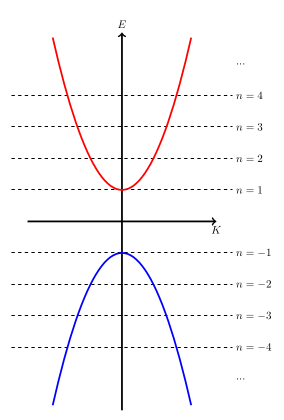
\includegraphics[width=3cm,height=4.5cm]{graficas/LL_material.png}
			\caption{\scriptsize{Niveles de Landau en material convencional}}
	\end{figure}
	\end{multicols}
\end{frame}

\begin{frame}{Niveles de Landau en el grafeno}
	\begin{multicols}{2}
		\scriptsize{En el grafeno, los niveles de Landau se pueden obtener a partir de considerar el hamiltoniano, 
						$\hat{H}=\frac{\hat{\pi}^2}{2m}+V(\vec{r})$ siendo $\pi=\vec{p}-e/c\vec{A}$ y $\vec{A}$ es el potencial vector, de la forma:
			\begin{equation}
					\hat{H} = \sqrt{\frac{2e\hbar B \nu_f}{c}}
					\left( \begin{array}{c c}
							0&\hat{a}\\\hat{a}^\dagger&0
					\end{array} \right)
			\end{equation}
			donde $\hat{a}= \sqrt{c/2e\hbar B}(\pi_x-i\pi_y)$ y 	$\hat{a}^\dagger=\sqrt{c/2e\hbar B}(\pi_x+i\pi_y)$. Resolviendo la ecuación de Schrödinger
			se obtiene que los niveles de energía vienen dados por:
			\begin{equation}
					E_n= \pm \hbar\omega_c \sqrt{n}
			\end{equation}
			donde $\omega_c = \sqrt{2}\nu_f/l_B$ es el ciclotrón cuántico y $l_B = \sqrt{\frac{\hbar c}{e B}}$ es la longitud magnética.}
		\begin{figure}
			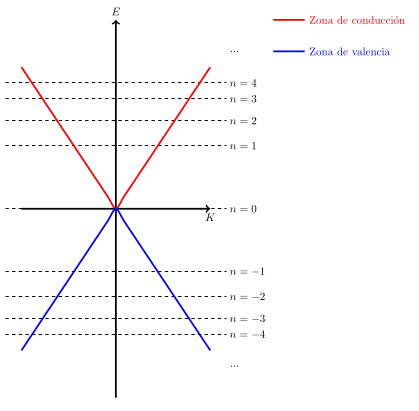
\includegraphics[height=4.5cm]{graficas/LL_grafeno.png}
			\caption{\scriptsize{Niveles de Landau en el grafeno}}
		\end{figure}
	
	\end{multicols}
	\end{frame}
\subsection{Estados de Bloch en grafeno en un campo eléctrico}

\begin{frame}
\end{frame}
\begin{frame}
\end{frame}
\begin{frame}
\end{frame}
\begin{frame}
\end{frame}

\begin{frame}
\end{frame}
\begin{frame}
\end{frame}
\begin{frame}
\end{frame}
